\documentclass[a4paper,12pt]{article}

\usepackage[utf8]{inputenc}
\usepackage[T1]{fontenc}
\usepackage[ngerman]{babel}
\usepackage{graphicx}
\usepackage{amsmath,amsthm, amssymb}
\usepackage{mathtools}
\usepackage{xcolor}
\usepackage{minted}
\usepackage{lmodern}
\usepackage[a4paper,margin=2.5cm]{geometry}
\usepackage{fancyhdr}
\usepackage{setspace}
\usepackage{caption}
\usepackage{subcaption}
\usepackage{nicefrac}
\usepackage{hyperref}

% Minted customization to remove background
\usemintedstyle{vs} % Visual Studio-like
\setminted{
    bgcolor=white, % ensures white background
    frame=lines,
    framesep=2mm,
    baselinestretch=1.2,
    fontsize=\footnotesize,
    linenos
}

\theoremstyle{definition}
\newtheorem{example}{Example}

\newcommand{\bigO}{\mathcal{O}}

\pagestyle{fancy}
\fancyhf{}
\lhead{PS Einführung in die Kryptographie}
\rhead{Andreas Schlager}
\cfoot{\thepage}

\title{Aufgabenblatt 08\\\large PS Einführung in die Kryptographie}
\author{Andreas Schlager}
\date{\today}

\onehalfspacing

% Theorem-Umgebung für Aufgaben
\newtheorem{aufgabe}{Aufgabe}

% ---- Makro für neue Aufgabe ----
\newcommand{\newaufgabe}[1]{
  \newpage
  \begin{aufgabe}
  #1
  \end{aufgabe}
  \addcontentsline{toc}{section}{Aufgabe \theaufgabe}
}

\begin{document}

\maketitle
\tableofcontents
\newpage

% Startnummer anpassen (z.B. erste Aufgabe hat Nummer 20, dann counter auf 19 setzen)
\setcounter{aufgabe}{26}

% ---- Aufgaben ----
\newaufgabe{Zur Known-Plaintext Attacke gegen 2 Key EDE TripleDES (Slide 138f): 
Erklären/beweisen
sie die angegebene Angriffskomplexität / Laufzeit der Oorschot, Wiener Attacke und
die Anzahl der im Mittel notwendigen Versuche für a. Hinweis: sehen sie sich die
Originalarbeit dazu an.}
\paragraph{Zeitkomplexität}
Zur Berechnung der asymptotischen Zeitkomplexität des Angriffs, wird für jeden 
Teilschritt die Komplexität angegeben.
\begin{enumerate}
    \item Gegeben eine Tabelle mit Plaintext- und Ciphertext Paaren
          (Tabelle 1, sortiert nach Plaintexten).
          \begin{enumerate}
            \item Sortieren benötigt bei $p$ Paaren $\bigO (p\log p)$.
          \end{enumerate}
    \item Erraten/wählen Sie einen fixen ersten Zwischenwert $a = E_{K_1}(P)$.
          \begin{enumerate}
            \item Ein fixes $a$ wählen geht in $\bigO (1)$.
          \end{enumerate}
    \item Bestimmen sie durch die Berechnung von $P = D_{K_1} (a)$ den
          Plaintext und suchen den dazugehörenden Ciphertext $C$ in Tabelle
          1, dies für alle $K_1$.
          \begin{enumerate}
            \item Pro $K_1$:
            \begin{enumerate}
                \item Berechnung von $P = D_{K_1} (a)$ in $\bigO (1)$.
                \item In der Tabelle suchen $\bigO (\log p)$.
            \end{enumerate}
            \item Insgesamt gibt es für $K \in \{0, 1\}^n$ $2^n$ Durchläufe. 
          \end{enumerate}
          Somit ist die Gesamtkomplexität für diesen Schritt $\bigO(2^n\log p)$.
    \item Tabulieren Sie für alle $K_1$ (für das fixe $a$) den zweiten
          Zwischenwert, $b = D_{K_1} (C)$ (Tabelle 2).\vspace*{1em}\\
          Entspricht wieder einem gesamten Durchlauf der Schlüssel ($2^n$). Bei jedem wird
          $b$ in $\bigO(1)$ berechnet. Die Komplexität beträgt daher $\bigO(2^n)$.
    \item Suchen Sie in der Tabelle 2 für alle möglichen $K_2$ Elemente mit
          passendem zweiten Zwischenwert $b = D_{K_2} (a)$.
          \begin{enumerate}
            \item Pro $K_2$:
            \begin{enumerate}
                \item Berechne $b = D_{K_2}(a)$ in $\bigO(1)$.
                \item Prüfe $b$ in Tabelle 2 (angenommen Hashtabelle) in $\bigO(1)$.
            \end{enumerate}
            \item Insgesamt gibt es wieder $2^n$ $K_2$, also auch $2^n$ Durchläufe.
          \end{enumerate}
          Gesamtkomplexität ist $\bigO(2^n)$.
    \item Bei Übereinstimmung ist ein mögliches Schlüsselpaar gefunden
          (mit weiteren Plaintext / Ciphertextpaaren verifizieren). Ansonsten
          wird ein neues $a$ gewählt.\vspace*{1em}\\
          Verifikation durch $p$ bekannte Paare in $\bigO(p)$.
\end{enumerate}
Durch die Schritte 3, 4 \& 5 ergeben sich folgende Laufzeiten
\[
    \bigO(2^n\log p), \bigO(2^n), \bigO(2^n).
\]
Im schlechtesten Fall müssen alle Zwischenwert für $a\in\{0,1\}^m$ überprüft werden.
\[
    \bigO(2^n\cdot 2^m) = \bigO(2^{n + m})
\]
\paragraph{Wahrscheinlichkeit} Es existieren $2^m$ mögliche Werte für $a$. In 
der Datenbank befinden sich $p$ Einträge. Unter der Annahme, dass jeder
Zwischenwert der Klartextpaare gleichverteilt ist, ist die Wahrscheinlichkeit einen
Treffer zu landen 
\[
    P(\text{Treffer})=\frac{p}{2^m}.
\]
Nimmt man dieses Wahrscheinlichkeit als die Wahrscheinlichkeit für ein Bernoulli-Experiment an,
gibt uns die geometrische Verteilung den Erwartungswert für die Anzahl $N$ an unterschiedlichen
Werten für $a$.
\[
    \mathbb{E}[N] = \frac{1}{P(\text{Treffer})} = \frac{2^m}{p}
\]
Im Schnitt müssen wir also nicht alle $2^m$ Werte für $a$ probieren (wie im worst-case),
sondern nur $\mathbb{E}[N]$ viele. Die erwartete Laufzeitkomplexität ist
\[
    \bigO\left(2^n\cdot \frac{2^m}{p}\right) = \bigO\left(\frac{2^{n + m}}{p}\right) 
\]
\paragraph{Fazit}
Je größer die Datenbank an Plaintext-Ciphertext-Paaren ist, desto schneller geht der Angriff.

\newaufgabe{Erklären sie warum die Berechnung von Diskrete Logarithmen und 
Quadratwurzeln in Modulararithmetik “computationally infeasible” ist, 
während in klassischer Arithmetik die entsprechenden Berechnungen 
nicht besonders aufwändig sind.}
\paragraph{Diskreter Logarithmus}
Der diskrete Logarithmus einer Zahl $m$ zur Basis $a$ modulo $p$ ist der kleinste Exponent
$x$ der Gleichung
\[
    a^x\equiv m \mod p.
\]
Das Problem bei der Berechnung ist, dass die Funktion $f(x) = a^x \mod p$ aufgrund
der Modulararithmetik nicht stetig wächst oder fällt. Die Ergebnisse für unterschiedliche
$x$ springen ohne klare Richtung. Somit kann man sich der korrekten Lösung
nicht annähern und es bleibt nur eine Brute-Force-Approach.
\begin{example}
    Sei $m = 3, p = 11$ und $a=2$.\footnote{Werte und Zahlen von \href{https://de.wikipedia.org/wiki/Diskreter_Logarithmus\#Beispiel}{Wikipedia} übernommen und nachgerechnet.}
    Man sieht in den Ergebnissen kein klar erkennbares Muster.
    \begin{figure}[h!]
        \centering
        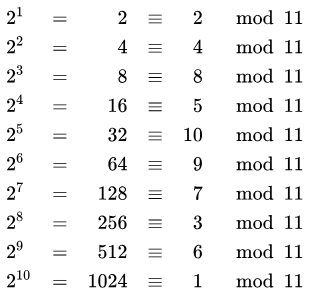
\includegraphics[width=0.4\textwidth]{img/discrete_log.png}
    \end{figure}
\end{example}
\paragraph{Quadartwurzel}
Das ziehen der Quadartwurzel bereitet im Restklassenringen mehrere Schwierigkeiten.
Eine davon ist, dass viele Zahlen überhaupt keine Wurzel besitzen.
Betrachtet man etwa den Restklassenring $\mathbb{Z}_7$ und sucht $x$, sodass
$x^2\equiv 3\mod 7$, wird man keine Lösung finden (siehe Tab \ref{ref:root_example}).
\begin{table}[htbp]
    \centering
    \begin{tabular}{c|c}
        $x$ & $x^2\mod 7$\\\hline
        0 & 0\\
        1 & 1\\
        2 & 4\\
        3 & 2\\
        4 & 2\\
        5 & 4\\
        6 & 1
    \end{tabular}
    \caption{Ergebnisse für $x^2$ in $\mathbb{Z}_7$}
    \label{ref:root_example}
\end{table}
Besonders interessant ist allerdings auch, dass sich das Ziehen der Quadartwurzel
im Restklassenring auf das Faktorisierungsproblem reduzieren lässt, welches
bekanntlich in NP liegt.
\newaufgabe{Erklären sie (und rechnen sie ein konkretes Beispiel durch), 
wie modulare Inversion
mit dem erweiterten Euklidischen Algorithmus realisiert werden kann.}
Der erweiterte euklidische Algorithmus berechnet für zwei Zahlen $a,b\in\mathbb{N}$
den größten gemeinsamen Teiler $\gcd(a,b)$. Außerdem liefert der Algorithmus zwei
weitere Zahlen $s,t\in\mathbb{Z}$, sodass der größte gemeinsame Teiler als Linearkombination
dieser Zahlen geschrieben werden kann (Lemma von Bézout).
\[
    \gcd(a,b) = s\cdot a + t \cdot b
\]
Das modulare Inverse einer Zahl $a\in \mathbb{N}$ ist eine Zahl $x\in\mathbb{Z}_n$, sodass
\[
    a\cdot x \equiv 1 \mod n.
\]
Um $x$ zu bestimmen, berechnet man zuerst über den erweiterten euklidischen Algorithmus
das Tupel $(\gcd(a, n), s, t)$. Ein modulares Inverses existiert genau dann, wenn
$\gcd(a,n) = 1$ (also $a$ und $n$ teilerfremd sind). Nach dem Lemma, lässt sich
der größte gemeinsame Teiler dann wie folgt schreiben.
\begin{align*}
    \gcd(a,n) = 1 &= s\cdot a + t\cdot n\\
    1 &\equiv s\cdot a + t\cdot n\mod n\\
    1 &\equiv s\cdot a\mod n
\end{align*}
Somit ist $s$ das modulare Inverse zu $a$ modulo $n$.
\paragraph{Algorithmus} Pseudocode des erweiterten euklidischen Algorithmus
\footnote{\href{https://de.wikipedia.org/wiki/Erweiterter_euklidischer_Algorithmus\#Rekursive_Variante}{Wikipedia, rekurisver, erweiterter euklidischer Algorithmus}}
\begin{figure}[h]
    \centering
    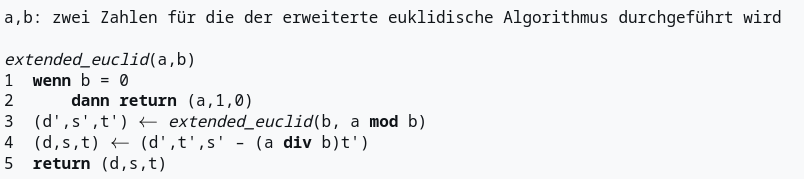
\includegraphics[width=\textwidth]{img/extended_euclid.png}
    \label{ref:ext_euclid}
\end{figure}\newpage
\begin{example}
    Seien $a = 7, n = 15$. Zuerst berechnet man den größten gemeinsamen Teiler
    wie beim regulären euklidischen Algorithmus.
    $q$ ist dabei das Ergebnis der ganzzahligen Division von $a$ und $n$.
    \begin{center}
        \begin{tabular}{|l|c|c|c|c|c|}
            \hline 
            Iteration & a & n & q\\
            \hline
            1 & 7 & 15 & 0 \\
            2 & 15 & 7 & 2 \\
            3 & 1 & 1 & 1 \\
            4 & 1 & 0 &\\
            \hline
        \end{tabular}
    \end{center}
    Sobald $n=0$ ist, steht in $a$ der ggT.
    Beginnend vom Tabellenende werden nun $s,t$ berechnet. Dafür soll in jeder Zeile $1 = s\cdot a + t\cdot n$ gelten.
    Dementsprechend wird in der letzten Zeile für $s = 1$ und $t=0$ eingetragen.
    Nun arbeitet man sich in der Tabelle hoch und berechnet die weiteren $s,t$ wie folgt
    \begin{align*}
        s &= t_{\text{alt}}\\
        t &= s_{\text{alt}} - q \cdot t_{\text{alt}}.
    \end{align*}
    Das $q$ ist immer aus der aktuellen Zeile.
    \begin{center}
        \begin{tabular}{|l|c|c|c|c|c|}
            \hline 
            Iteration & a & n & q & s & t\\
            \hline
            1 & 7 & 15 & 0 & -2 & 1\\
            2 & 15 & 7 & 2 & 1 & -2 \\
            3 & 1 & 1 & 1 & 0 & 1 \\
            4 & 1 & 0 & & 1 & 0\\
            \hline
        \end{tabular}
    \end{center}
    In der obersten Zeile steht nun das Ergebnis für $s,t$. 
    \[
        \gcd(7, 15) = 1 = -2\cdot 7 + 1\cdot 15
    \]
    Entsprechend der obigen Erklärung wäre das modulare Inverse zu $7\mod 15$ also $-2$.
    \[
        7\cdot (-2)\equiv 1 \mod 15
    \]
\end{example} 
\newaufgabe{Beweisen Sie: Ist $n=p\cdot g$ mit $p,g\in \mathbb{P}$: $\phi(n) = (p - 1)(g - 1)$.}
\begin{proof}
    $\phi(n) = (p - 1)(g - 1)$.

    $n$ ist eine zusammengesetzte Zahl, deren Primfaktorenzerlegung 
    genau $p \cdot g$ ist. Somit sind alle Vielfachen der Primzahlen, die
    nicht größer als $n$ sind, \textbf{nicht} teilerfremd zu $n$ (der gemeinsame Teiler
    sind die entsprechenden Primzahlen). 
    \begin{align*}
        \vert 
        \{
            k\cdot p \mid 1 \leq k \leq g 
        \} \vert = \vert \{
            p, 2p, 3p, \dots, g\cdot p
        \}\vert &= g\\
        \vert
        \{
            k\cdot g \mid 1 \leq k \leq p 
        \} \vert = \vert \{
            g, 2g, 3g, \dots, p\cdot g
        \}\vert &= p
    \end{align*}
    Ausgehend von alle in Frage kommenden Zahlen $p\cdot g$, ziehen wir
    jeweils obigen Anzahl ab und achten darauf, die Schnittmenge ($n$) nur einmal
    abzuziehen.
    \begin{align*}
            \phi(n) &= p\cdot g - 1 - p + 1 - g + 1\\
            &= p\cdot g - p - g + 1\\
            &= (p - 1) (g - 1)
    \end{align*}
\end{proof}

\end{document}
